\documentclass[12pt,letter]{article}
\usepackage{tikz}
\usetikzlibrary{shapes,arrows}
\usepackage{float}
%defining tikz block characteristics
\tikzstyle{block} = [draw, fill=blue!20, rectangle, 
minimum height=3em, minimum width=6em]
\tikzstyle{sum} = [draw, fill=blue!20, circle, node distance=1cm]
\tikzstyle{input} = [coordinate]
\tikzstyle{output} = [coordinate]
\tikzstyle{pinstyle} = [pin edge={to-,thin,black}]

%opening
\title{\textbf{ECE 438 Homework \#5}}
\author{Adam Sumner}
\date{Monday April 27th, 2015}

\begin{document}

\maketitle
\section*{System Diagram}
\begin{figure}[H]
\centering
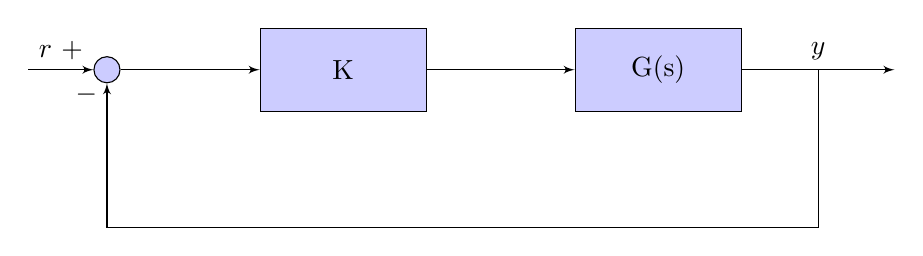
\begin{tikzpicture}[auto, node distance=2cm,>=latex']

% We start by placing the blocks
\node [input, name=input] {};
\node [sum, right of=input] (sum) {};
\node [block, right of =sum, node distance = 3cm] (controller) {K};
\node [block, right of=controller, node distance=4cm] (system) {G(s)};
% We draw an edge between the controller and system block to 
% calculate the coordinate u. We need it to place the measurement block. 
\draw [->] (controller) -- node[name=u] {} (system);
\node [output, right of=system, node distance = 3cm] (output) {};


% Once the nodes are placed, connecting them is easy. 
\draw [draw,->] (input) -- node {$r$ $+$} (sum);
\draw [->] (sum) -- node {} (controller);
\draw [->] (system) -- node [name=y] {$y$}(output);
\draw [->] (y.south) |- ++(0,-2cm)  -| node[pos=.96]{$-$}(sum) ;
%node [near end] {$y_m$} (sum);
\end{tikzpicture}
\end{figure}

$$G(s)= \frac{1}{s(s+5)(s^2+4s+20)}$$

\section*{Task 1}
When K = 10, KG(s) becomes $\frac{10}{s(s+5)(s^2+4s+20)}$. This equation has 2 real poles and 2 complex poles at 0, -5, and -2 $\pm$ 4j. Converted into standard form we get:
$$KG(s) = \frac{1}{10} \cdot \frac{1}{s(\frac{s}{5}+5)(\frac{s^2}{20}+\frac{s}{5}+1)}$$

$$Peak\hspace{.1cm}height = -20log_{10}\left(2\zeta\sqrt{1-\zeta^2}\right) \approx 1.93dB$$

\noindent For complex conjugate poles, a common way to express a second order polynomial is:
$$\left( \frac{s}{\omega_0}\right)^2+2\zeta\left(\frac{s}{\omega_0}\right)+1$$
$$\omega_0=\sqrt{20} \approx 4.4721, \zeta = \frac{\sqrt{20}}{10} \approx 0.44721$$

\noindent With this information we can draw our bode plot as such:

\begin{figure}[H]
\centering
\includegraphics[width=1\linewidth]{Task1}
\caption{Hand Drawn Bode Plot of $KG(s)$}
\label{fig:Task1}
\end{figure}

\section*{Task 2}
Using the bode plot from Task 1, we can pick points and calculate values to construct the Nyquist plot:

\begin{figure}[H]
\centering
\includegraphics[width=1\linewidth]{"Task 2"}
\caption{Hand Drawn Nyquist Plot}
\label{fig:Task2}
\end{figure}

\section*{Task 3}


\begin{figure}[H]
\centering
\includegraphics[width=1\linewidth]{Task3}
\caption{Matlab Bode Plot}
\label{fig:Task3}
\end{figure}

\noindent Where the gain margin is 30.1 dB at 3.33 rad/s and the Phase margin is 87.7 degrees at 0.1 rad/s.
\section*{Task 4}
\begin{figure}[H]
\centering
\includegraphics[width=1\linewidth]{Task4}
\caption{Matlab Nyquist Plot}
\label{fig:Task4}
\end{figure}


\section*{Task 5}
At the point (-1,0) there are no loops therefore N = 0 and Z = 0, so P = 0. This system is stable for K = 10.

\section*{Task 6}
Our phase margin is 30.1dB which corresponds to $20log(x)=30.1$. Solving for x we get 31.988. 1/31.988 gives us $\approx$ 0.0312. It is clear that the Nyquist plot crosses the negative real axis at 0.0312. Because our gain margin is 30.1db, our maximum gain for stability will be 31.988 times our original system gain. This gives us a maximum gain of 319.88. So for $0< K < 319.88$, the system is stable.
\section*{Task 7}
Let's analyze the root locus of this system.

\section*{Task 8}
We will first plot the root locus of the system, then analyze the system when the poles are in the right half side of the plane. The gain at the point when the poles are in the right half side of the plane will be the maximum gain the system can have to maintain stability.

\section*{Task 9}

\begin{figure}[H]
	\centering
	\includegraphics[width=1\linewidth]{"Task 7"}
	\caption{Root Locus of System}
	\label{fig:Task7}
	\end{figure}
	
	\noindent It can clearly be seen that as soon as the gain of the system is $\approx$ 32, the system becomes unstable. Multiplying 32 by our original gain of 10, we obtain a total value of K to be 320. This directly supports our Nyquist analysis that the system is stable for $0 < K < 320$.
\end{document}
